\documentclass[12pt]{article}
\usepackage{amsmath,mathtools}
\usepackage[usenames,dvipsnames]{xcolor}
\usepackage{textcomp}
\usepackage{cmbright}
\usepackage[german]{babel}
\usepackage{microtype}
%\usepackage{microtype}
\usepackage[utf8]{inputenc}
\usepackage[T1]{fontenc}
\usepackage{helvet}
\renewcommand{\familydefault}{\sfdefault}

\usepackage{siunitx}
%\usepackage{tikz}
\usepackage{fancyhdr}
\usepackage{sectsty}
\usepackage{setspace}
\usepackage{booktabs} % To thicken table lines
\usepackage[version=4]{mhchem}
\usepackage{textcomp}
\usepackage{tabularx}

%\usepackage[pass]{geometry}
%\usepackage[compatibility=4.7,language=german]{chemmacros}

\usepackage[ddmmyyyy]{datetime}
\renewcommand{\dateseparator}{.}

\pagestyle{fancy}

\cfoot{\thepage}

\lhead{Nevroz Arslan }
\rhead{\today}
\setlength{\headheight}{15pt}

\usepackage{overcite}
\renewcommand\citeform[1]{[#1]}

%\renewcommand*\printatom[1]{{\fontsize{10}{12}\selectfont\ensuremath{\mathsf{#1}}}}
\sectionfont{\fontsize{12}{15}\selectfont}

\makeatletter
    \setlength\@fptop{0\p@}
\makeatother


\newcommand\textbox[1]{%
  \parbox{.333\textwidth}{#1}%
}


\setlength{\headheight}{15pt}
\sisetup{detect-weight=true, detect-all}
\sisetup{text-celsius = $^\circ\mkern-1mu$C}

\renewcommand{\thesection}{\arabic{section}.}
\renewcommand{\thesubsection}{\thesection\arabic{subsection}}
\renewcommand{\headrulewidth}{0pt}

\begin{document}

\begingroup
\leftskip=0cm plus 0.5fil \rightskip=0cm plus -0.5fil
\parfillskip=0cm plus 1fil
 \textbf{\large Darstellung von (\textit{4R,5R})-4,5-Bis(chlordiphenylmethyl)-2,2-dimethyl-1,3-dioxolan}\par
\endgroup

\begin{center}
 \textbf{Präparat Nr. 4 von 7}
\end{center}
\section{Reaktionstyp: \textnormal{Innere nucleophile Substitution} }
\begin{figure}[ht]
\centering
\includegraphics[width=\textwidth]{reaktion.png}
\end{figure}

%\chemabove{\lewis{2:,Si}}{\hspace{5mm}\scriptstyle\ominus}
%%%%%%%%%%%%%
% Berechnung des Ansatzes
%%%%%%%%%%%%%
\begin{onehalfspace}

\section{Berechnung des Ansatzes: }
Es sollte (\textit{4R,5R})-4,5-Bis(chlordiphenylmethyl)-2,2-dimethyl-1,3-dioxolan aus (\textit{4R,5R})-2,2-Dimethyl-$\alpha ,\alpha ,\alpha ',\alpha '$-tetraphenyl-1,3-dioxolan-4,5-dimeth-\\anol (1.30 \si{\gram}, 2.8 mmol) hergestellt werden. Die Umrechnung des Literaturansatzes ergab folgenden Ansatz:\cite{vor}

\begin{table}
\begin{tabularx}{\textwidth}{Xrrrr}
\toprule
\textbf{ Bezeichnung }&\textbf{M [\si{\gram\per\mol}]} & \textbf{ n [\si{\milli\mol}]} & \textbf{Menge} & \textbf{Equiv}\\
\midrule
(\textit{4R,5R})-2,2-Dimethyl-$\alpha ,\alpha ,\alpha ',\alpha '$-tetraphenyl-1,3-dioxolan-4,5-dimethanol & 466.57 & 2.8  & 1.30 \si{\gram} & 1.00 \\
 Thionylchlorid  & 118.97   &  8.4  &  0.6 \si{\milli\liter} & 3.00 \\
 Triethylamin    & 101.19   &  14.0 &  2.0 \si{\milli\liter} & 5.00 \\
 Dichlormethan &   &  & 80 \si{\milli\liter}& LM \\
\bottomrule
\end{tabularx}\\
\end{table}

%%%%%%%%%%%%%
% Durchführung
%%%%%%%%%%%%%
\section{Durchführung \cite{vor}}
In einem 500 \si{\milli\liter} Dreihalskolben, ausgestattet mit Tropftrichter und Rückflusskühler, wurden (\textit{4R,5R})-2,2-Dimethyl-$\alpha ,\alpha ,\alpha ',\alpha '$-tetraphenyl-1,3-diox-olan-4,5-dimethanol (1.30 \si{\gram}, 2.8 \si{\milli\mol}) und Thionylchlorid (0.6 \si{\milli\liter}, 8.4~\si{\milli\mol}) in Dichlormethan (25 \si{\milli\liter}) vorgelegt. Zu dieser Lösung wurde innerhalb von 20 Minuten Triethylamin (2.0 \si{\milli\liter}, 14.0 \si{\milli\mol}) in Dichlormethan (25~\si{\milli\liter}) zugetropft und das Reaktionsgemisch wurde anschließend unter Rückfluss 30 Minuten erhitzt. Danach wurde zum Reaktionsgemisch \ce{NaHCO_3} (gesättigt, 100 \si{\milli\liter}) hinzugegeben und noch 4 Stunden bei 10 \si{\celsius} gerührt. Die organische Phase wurde abgetrennt, über Magnesiumsulfat getrocknet und am Rotationsverdampfer eingeengt. Der Rückstand wurde aus Heptan umkristallisiert.
%Das Produkt (7.94 \si{\gram}, 17 \si{\milli\mol}, 68 \%) wurde als gelber Feststoff erhalten.
\section{Fehlerbetrachtung}

Die Synthese von (\textit{4R,5R})-4,5-Bis(chlordiphenylmethyl)-2,2-dimethyl-1,3-dioxolan wurde zweimal durchgeführt. 
Laut den NMR-Messungen wurde das gewünschte Produkt in beiden Fällen nicht erhalten.
Bei der ersten Durchführung war eine Unstimmigkeit zu beobachten. 
Das eingesetzte Thionylchlorid hat beim Vorlegen in dem Kolben sofort reagiert was an der Bildung von weißem dichten Nebel zu sehen war. Dies hätte erst bei der Zugabe von Triethylamin zum Reaktionsgemisch passieren sollen. Der entstandene Fehler ist auf einen undichten Apparaturaufbau zurückzuführen, der kleine Mengen Triethylamin ins Reaktionsmilieu einsickern lassen haben könnte. 
Bei der zweiten Durchführung trat dieser Fehler nich auf, allerdings hat die Umsetzung nicht zum gewünschten Produkt geführt.
Die NMR-Messungen weisen auf das monosubstituierte Produkt hin. Es könnte sein, dass eine vollständige Umsetzung durch eine frühzeitige Beendigung der Reaktion verhindert wurde. Des weiteren könnte das eingesetzte Thionylchlorid oder Triethylamin schon zu alt gewesen sein.

\section{Mechanismus\cite{organikum}}
Die Darstellung von Alkylhalogeniden mit Hilfe des Thionylchlorids (\textbf{2}) läuft nach einem internen \ce{S_N}i Mechanismus ab.
Im ersten Schritt der Reaktion greift das Sauerstoffatom des Alkohols \textbf{1} das Thionylchlorid (\textbf{2}) an. Es bildet sich eine dipolare Zwischenstufe \textbf{3}, welche unter Abspaltung eines Chlorids in das Kation \textbf{4} umgewandelt wird. Im folgenden Schritt deprotoniert das Triethylamin (\textbf{5}) das Kation \textbf{4}, wobei unter Bildung eines stabilen Salzes \textbf{6} ein Schwefligsäureester \textbf{7} entsteht. 
Danach erfolgt eine intramolekulare nukleophile Substitution, bei der das Chlor auf den Kohlenstoff der ehemaligen Alkoholfuntion übertragen wird und gleichzeitig \ce{SO_2} abgespalten wird. Es bildet sich  das gewünschte Produkt (\textit{4R,5R})-4,5-Bis(chlordiphenylmethyl)-2,2-dimethyl-1,3-dioxolan (\textbf{8}).\\

\begin{figure}[!htbp]
\centering
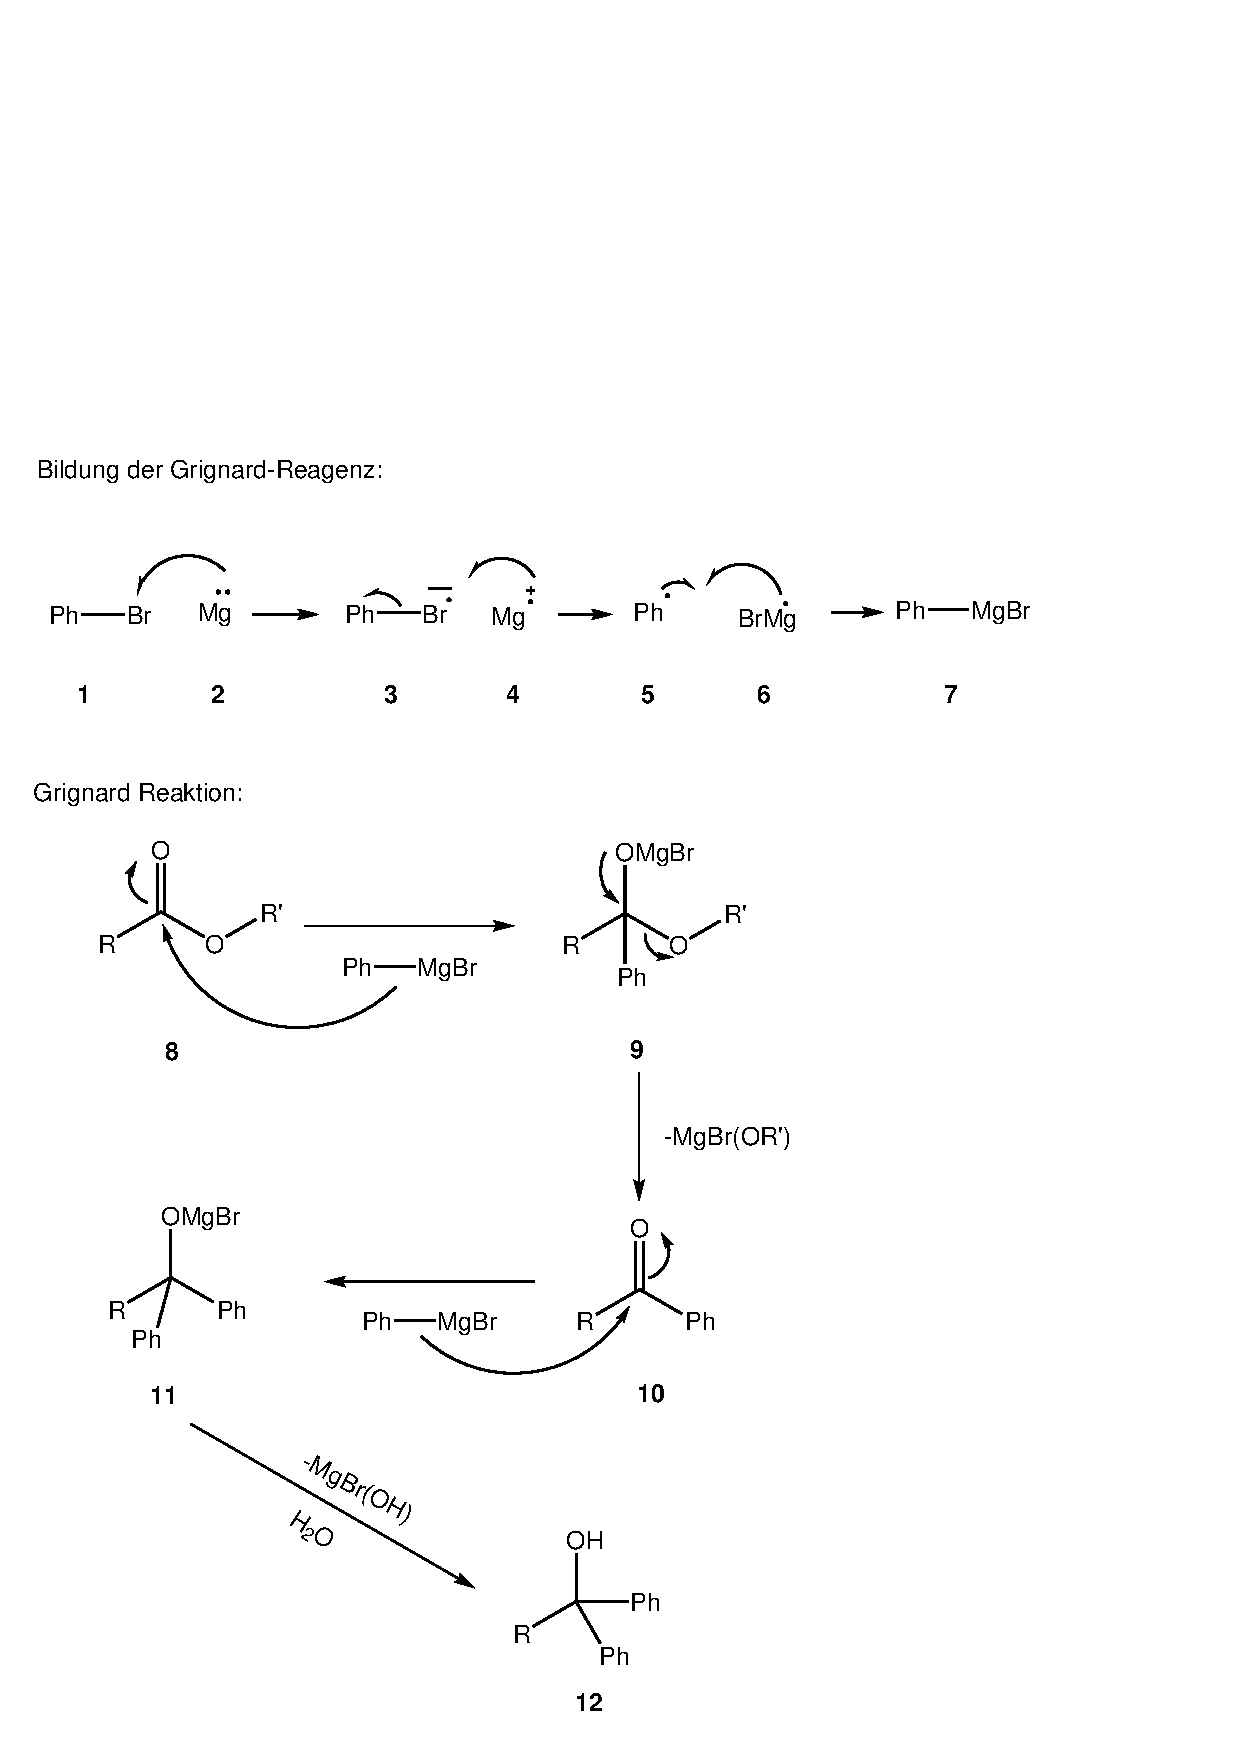
\includegraphics[width=\textwidth]{mechan.png}
\end{figure}
\newpage    

\section{Abfallentsorgung}
Die nach dem Hydrolysieren verbleibenden wässrigen Phasen wurden
nach einer pH-Wertbestimmung im Behälter für basische wässrige Abfälle entsorgt.
Das im Rotationsverdampfer abgetrennte Lösungsmittel wurde im Behälter für halogenhaltige Kohlenwasserstoffe entsorgt.
\section{Literatur}

\renewcommand{\section}[2]{}%
\def\bibindent{0em}
\begin{thebibliography}{99\kern\bibindent}
\makeatletter
\let\old@biblabel\@biblabel
\def\@biblabel#1{\old@biblabel{#1}\kern\bibindent}
\let\old@bibitem\bibitem
\def\bibitem#1{\old@bibitem{#1}\leavevmode\kern-\bibindent}
\makeatother
\bibitem{vor}
R. Hilgraf, A. Pfalz, \textit{Adv. Synth. Catal.} \textbf{2005}, \textit{37}, 61 - 77.
\bibitem{organikum}
K. Schwetlick, \textit{Organikum}, 21. Aufl., Wiley-Vch, Weinheim \textbf{2001}, S. 230.
\end{thebibliography}
\end{onehalfspace}
\end{document}


